\documentclass[letter, 12pt]{article}

\usepackage{amsmath,amsthm,amssymb}
\usepackage{fancyhdr}
\usepackage{geometry}
\usepackage{enumerate}
\usepackage{enumitem}
\usepackage{listings}
\usepackage{algorithm}
\usepackage{hyperref}
\usepackage{algorithmic}
\usepackage{eqparbox}
\usepackage{float}
\usepackage{bm}
\usepackage{bbm}
\usepackage{mathtools}
\usepackage{minted}
\usepackage{forest}

\author{Shengjie Li}
\title{CS 536 : Decision Trees}

\pagestyle{fancy}
\fancyhf{} 
\lhead{Shengjie Li \\ RUID: 188008047}
\cfoot{\thepage} 
\renewcommand{\headrulewidth}{1pt}
\renewcommand{\headwidth}{\textwidth}
\renewcommand\algorithmiccomment[1]{%
    \hfill\#\ \eqparbox{COMMENT}{#1}%
}
\newlist{subquestion}{enumerate}{1}
\setlist[subquestion, 1]{label = \alph*)}
\DeclareMathOperator*{\argmax}{arg\,max}
\DeclareMathOperator*{\argmin}{arg\,min}

\setlength\parindent{0pt}

% margin adjustment
\addtolength{\textwidth}{1in}
\addtolength{\oddsidemargin}{-0.5in}
\addtolength{\evensidemargin}{-0.5in}
\addtolength{\topmargin}{-.5in}
\addtolength{\textheight}{1.0in}
\setlength\parindent{0cm}

\begin{document}
    \centerline{\textbf{CS 536 : Decision Trees}}
    \begin{enumerate}
        \item {For a given value of $ k, m $, (number of features, number of data points), write a function to generate a training
            data set based on the above scheme.}
        \begin{minted}{python}
def get_data(k, m, save = False):
    # input args:
    # k: number of features
    # m: number of data points
    X = np.zeros((m, k))
    Y = np.zeros((m, 1))
    w = np.zeros(k)
    denom = 0.9 * 10 * (1 - (0.9 ** (k - 1)))
    for j in range(m):
        s = 0
        if np.random.rand() >= 0.5:
            X[j][0] = 1
        for i in range(1, k):
            if np.random.rand() >= 0.75:
                X[j][i] = X[j][i - 1]
            else:
                X[j][i] = 1 - X[j][i - 1]
            w[i] = (0.9 ** i) / denom
            s += w[i] * X[j][i]
        if s >= 0.5:
            Y[j] = X[j][0]
        else:
            Y[j] = 1 - X[j][0]
    if save == True:
        save_arr(np.concatenate((X, Y), axis = 1))
    return X, Y
        \end{minted}
        \item {Given a data set, write a function to fit a decision tree to that data based on splitting the variables by maximizing
            the information gain. Additionally, return the training error of this tree on the data set, $ err_{train} (\hat{f}) $. \textit{It may be
            useful to have a function that takes a data set and a variable, and returns the data set partitioned based on the
            values of that variable.}}
        \begin{minted}{python}
import numpy as np

eps = 1e-5

class Node:
    x_id = None
    y = None
    equals_zero = None
    equals_one = None
    def __init__(self, x_id):
        self.x_id = x_id

class DecisionTree:
    root = None
    def __init__(self):
        self.root = Node(None)

def entropy(P, P_y0):
    if P < eps or P > 1 - eps or P_y0 < eps or P_y0 > 1 - eps:
        return 0
    return -P * np.log(P) - P_y0 * np.log(P_y0)

def IC(X, Y):
    m = X.shape[0]
    x_1 = np.count_nonzero(X)
    if x_1 == 0 or x_1 == m:
        return 0
    c_00 = 0
    c_01 = 0
    c_10 = 0
    c_11 = 0
    for x, y in zip(X, Y):
        if x < eps:
            if y < eps:
                c_00 += 1
            else:
                c_01 += 1
        else:
            if y < eps:
                c_10 += 1
            else:
                c_11 += 1
    P_x = x_1 / m
    P_00 = c_00 / (c_00 + c_01)
    P_01 = c_01 / (c_00 + c_01)
    P_10 = c_10 / (c_10 + c_11)
    P_11 = c_11 / (c_10 + c_11)
    return P_x * entropy(P_11, P_10) + (1 - P_x) * entropy(P_01, P_00)

def fit_decision_tree(X, Y, node, p_vis):
    m, k = X.shape
    P_y = np.count_nonzero(Y) / m
    H_y = entropy(P_y, 1 - P_y)
    maxx = 0
    max_id = -1
    vis = np.copy(p_vis)
    for i in range(k):
        if vis[i] == 1:
            continue
        IG = H_y - IC(X[:, i], Y)
        if IG > maxx:
            maxx = IG
            max_id = i
    if max_id != -1:
        vis[max_id] = 1
        new_X_0 = np.copy(X)
        new_X_1 = np.copy(X)
        new_Y_0 = np.copy(Y)
        new_Y_1 = np.copy(Y)
        for i in range(m - 1, -1, -1):
            if new_X_0[i][max_id] > 1 - eps:
                new_X_0 = np.delete(new_X_0, i, axis = 0)
                new_Y_0 = np.delete(new_Y_0, i, axis = 0)
            if new_X_1[i][max_id] < eps:
                new_X_1 = np.delete(new_X_1, i, axis = 0)
                new_Y_1 = np.delete(new_Y_1, i, axis = 0)
        node.x_id = max_id
        if new_X_0.shape[0] > 0:
            node.equals_zero = Node(None)
            fit_decision_tree(new_X_0, new_Y_0, node.equals_zero, vis)
        if new_X_1.shape[0] > 0:
            node.equals_one = Node(None)
            fit_decision_tree(new_X_1, new_Y_1, node.equals_one, vis)
    else:
        if P_y >= 0.5:
            node.y = 1
        else:
            node.y = 0
        \end{minted}
        \item {For $ k = 4 $ and $ m = 30 $, generate data and fit a decision tree to it. Does the ordering of the variables in the
            decision tree make sense, based on the function that defines Y ? Why or why not? Draw the tree.} 
        \par{\textbf{Solution:}}
        \par{The generated data looks like this:}
        \begin{lstlisting}[backgroundcolor = \color{lightgray}]
X = [1 0 0 1]   Y = 0
    [1 0 1 1]       1
    [1 0 0 1]       0
    [0 1 0 1]       0
    [0 1 0 0]       1
    [1 0 1 0]       0
    [0 1 1 0]       0
    [0 1 0 0]       1
    [0 0 1 0]       1
    [0 0 1 0]       1
    [1 0 1 0]       0
    [0 1 1 0]       0
    [1 1 0 1]       1
    [1 0 1 1]       1
    [1 0 0 1]       0
    [0 1 0 1]       0
    [0 1 0 0]       1
    [0 1 0 1]       0
    [0 0 0 1]       1
    [1 0 1 0]       0
    [0 1 1 0]       0
    [0 1 0 1]       0
    [1 1 0 1]       1
    [1 0 1 0]       0
    [0 1 1 0]       0
    [0 1 1 0]       0
    [1 1 1 0]       1
    [1 1 0 1]       1
    [0 1 0 1]       0
    [0 1 0 1]       0
        \end{lstlisting}
        \begin{center}
        	\begin{forest}
            for tree={circle,draw, l sep=20pt}
            [$ X_0 $
                [$ X_1 $, edge label={node[midway,left] {0}}
                    [\text{$ Y = 1 $}, edge label={node[midway,left] {0}}]
                    [$ X_3 $, edge label={node[midway,right] {1}}
                        [$ X_2 $, edge label={node[midway,left] {0}}
                            [\text{$ Y = 1 $}, edge label={node[midway,left] {0}}]
                            [\text{$ Y = 0 $}, edge label={node[midway,right] {1}}]
                        ]
                        [\text{$ Y = 0 $}, edge label={node[midway,right] {1}}]
                    ]
                ]
                [$ X_1 $, edge label={node[midway,right] {1}}
                    [$ X_3 $, edge label={node[midway,left] {0}}
                        [\text{$ Y = 0 $}, edge label={node[midway,left] {0}}]
                        [$ X_2 $, edge label={node[midway,right] {1}}
                            [\text{$ Y = 0 $}, edge label={node[midway,left] {0}}]
                            [\text{$ Y = 1 $}, edge label={node[midway,right] {1}}]
                        ]
                    ]
                    [\text{$ Y = 1 $}, edge label={node[midway,right] {1}}]
                ]
            ]
        \end{forest}
        \end{center}
    	\par{I think the ordering of variables of this decision tree kind of makes sense. Because the generation of $ X_i $ heavily depends on the previous value $ X_{i-1} $, it's intuitive to split the data in the order of $ X_0, X_1, X_2, X_3 $. Note that if the data point have more $ 1s $, the sum of $ w_2X_2 + w_3X_3 + \dots + w_kX_k$ would be relatively large. Thus, the leaves nodes with a path of more $ 1s $ are likely to have the different value than $ X_0 $, and vice versa.}
        \item {Write a function that takes a decision tree and estimates its typical error on this data $ err (\hat{f}) $; i.e., generate a
            lot of data according to the above scheme, and find the average error rate of this tree over that data.}
        \begin{minted}{python}
def predict(node, x):
    if node == None:
        return 1 # No data captured
    if node.y != None:
        return node.y
    if x[node.x_id] < eps:
        return predict(node.equals_zero, x)
    else:
        return predict(node.equals_one, x)

def get_err(tree, X, Y):
    s = 0
    m, k = X.shape
    for i in range(m):
        prediction = predict(tree.root, X[i])
        if prediction != Y[i]:
            s += 1
    print('Training error is: %f' % (1.0 * s / m))
    return 1.0 * s / m
        \end{minted}
        \par{I generated data of $ m = 10,000 $ and used the decision tree I got in the previous question to predict $ Y $ and get the error. I did this for $ 50 $ times and then got the average error: $ 0.046790 $.}
        
        \item {For $ k = 10 $, estimate the value of $ |err_{train} (\hat{f}) - err (\hat{f})| $ for a given $ m $ by repeatedly generating data sets, fitting
            trees to those data sets, and estimating the true and training error. Do this for multiple $ m $, and graph this
            difference as a function of $ m $. What can you say about the marginal value of additional training data?}
        \begin{figure}[H]
        	\centering
        	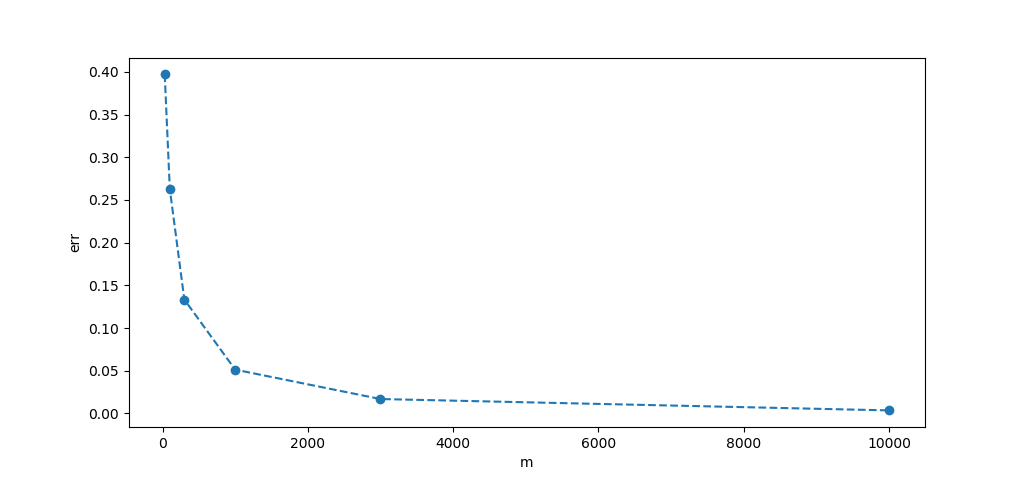
\includegraphics[width=\textwidth]{q5.png}
        	\label{fig:q5}
        	\caption{Differnt errors versus different ms}
        \end{figure}
    	\par{I did this experiment for $ m = 30, 100, 300, 1000, 3000, 10000 $. For every m, I generated 10 different training sets and fitted decision trees on these training sets, tested these decision trees on 10 different test sets of $ m = 10,000 $ and got the average errors. (100 tests for every m)}
    	\par{The average errors are: $ 0.396951, 0.262908, 0.133341, 0.051315, 0.016886, 0.003579 $, respectively.}
    	\par{Note that $ 2^k = 2^{10} = 1024 $, the larger the m is, the more likely we have got all possible combinations of $ X $.}
    	\par{From the \ref{fig:q5} we can see, the line tend to level out after $ m \ge 3000 $, thus I guess the marginal value of m is around $ 3000 $.}
    	
        \item {Design an alternative metric for splitting the data, not based on information content / information gain. Repeat
        	the computation from (5) above for your metric, and compare the performance of your trees vs the ID3 trees.}
        \par{\textbf{Solution:}}
        \par{I designed a pretty greedy yet simple metric: find the $ X $ that agrees on $ Y $ the most, i.e. \[ \argmax_{i} \max (\sum_{j=1}^{m}\mathbbm{1}X^j_i = Y^j, \sum_{j=1}^{m}\mathbbm{1}X^j_i \ne Y^j) \]}
        \par{The results are actually pretty good as \ref{fig:q6} shows.}
        \begin{figure}[H]
        	\centering
        	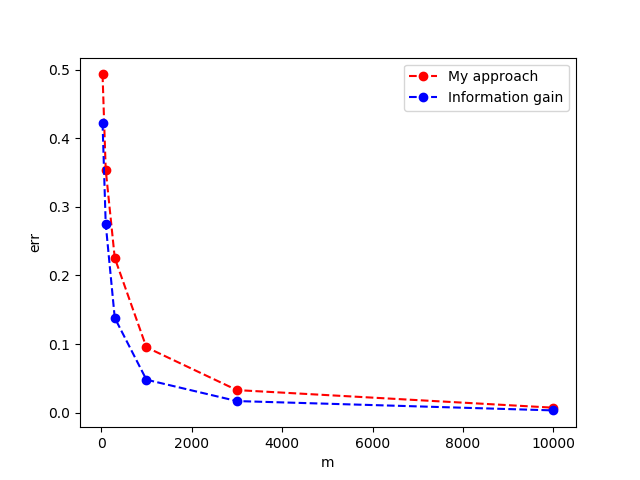
\includegraphics[width=\textwidth]{q6.png}
        	\label{fig:q6}
        	\caption{Comparison}
        \end{figure}
    \end{enumerate}
\end{document}
